\chapter{Theoretical Background and Related Work}
Detecting gender bias in English-German (EN-DE) translations using Natural Language Processing (NLP) requires an understanding of what gender bias means in this context, how it appears in MT, and how it has been studied so far. To build this foundation, this chapter (1) defines the concept of gender bias in machine translation, (2) outlines its relevance, (3) identifies gaps in current research, and (4) justifies the technical design decisions made in this project.

\vspace{1cm} 
\begin{figure}[htb]
    \centering
    \scalebox{0.8}{\tikzstyle{startstop} = [rectangle, rounded corners, minimum width=3.5cm, minimum height=1cm, text centered, draw=black, fill=gray!20]
\tikzstyle{process} = [rectangle, minimum width=3.5cm, minimum height=1cm, text centered, draw=black, fill=blue!10]
\tikzstyle{arrow} = [thick,->,>=stealth]

\begin{tikzpicture}[node distance=1.7cm]

\node (start) [startstop] {Define Key Concepts};
\node (review) [process, below of=start] {Review Related Work};
\node (gaps) [process, below of=review] {Identify Research Gaps};
\node (position) [process, below of=gaps] {Position Thesis Contribution};
\node (tech) [startstop, below of=position] {Explain Technical Approach};

\draw [arrow] (start) -- (review);
\draw [arrow] (review) -- (gaps);
\draw [arrow] (gaps) -- (position);
\draw [arrow] (position) -- (tech);

\end{tikzpicture}
}
    \caption{Overview of Chapter 2 Structure.}
    \label{fig:workflow_theory}
\end{figure}
\vspace{1cm} 

% --------------------------------------------------------------------------------

\section{Definitions}
\subsection{Natural Language Processing vs. Machine Translation}
    \textbf{NLP} refers to the development of machine systems that can process and generate human language. The goal is to mimic and understand it as fluently as possible \parencite{smacchiaDoesAIReflect2024,ullmannGenderBiasMachine2022}. Common applications are chatbots, translation tools, speech recognition, and image captioning.

    \textbf{MT} is a direct application of NLP. It enables the automatic translation of text from one language to another \parencite{linMachineTranslationAcademic2009}. Over time, MT systems have developed from rule-based and statistical approaches, which depend on hand-crafted grammar rules or aligned sentence data, into more adaptable neural models \parencite{chakravarthiSurveyOrthographicInformation2021}.

    Most modern systems, such as Google Translate and DeepL, rely on neural machine translation (NMT) \parencite{wuGooglesNeuralMachine2016,deeplHowDoesDeepL2021}. These models are trained on large collections of translated texts. They learn to represent the meaning of entire sentences as mathematical structures, enabling more fluent and accurate translations. Unlike earlier approaches, NMT systems take the full sentence context into account, which helps reduce errors and improves the handling of ambiguous or idiomatic language \parencite{wuGooglesNeuralMachine2016}. Throughout this work, all MT systems referenced or applied are neural models.

\subsection{Bias in Society and its Manifestations}
\label{subsection:manifestations_of_gb}
    Bias refers to a tendency to favour or disadvantage certain individuals or groups based on preconceived ideas. It often comes from stereotypes, which are fixed and oversimplified ideas about a group. While stereotypes describe assumptions about people, bias influences actual behavior and treatment.

    Bias takes many forms and can be based on characteristics such as age, disability, gender, ethnicity, religion, or sexual orientation \parencite{ullmannGenderBiasMachine2022}. These biases often originate from longstanding cultural and historical beliefs about the expected behavior of different groups.

    This study focuses specifically on gender bias. It is particularly prominent in machine translation due to the influence of gendered language. Elements such as gendered terms, occupational roles, and grammatical patterns can affect translations and often perpetuate stereotypes.
    
    Drawing on key studies that examine gender bias in EN-DE MT \parencite{ullmannGenderBiasMachine2022,rescignoGenderBiasMachine2023,lardelliBuildingBridgesDataset2024,kapplAreAllSpanish2025}, such bias typically manifests in the following forms:

    \subsubsection{Defaulting to Masculine Forms}
        In both singular and plural contexts, the \textit{generic masculine} refers to the default use of the masculine grammatical gender.
        For example, the sentence "Die Studenten sind im Hörsaal" (translation: "The students are in the lecture hall") uses the masculine plural form to refer to a group of students regardless of their gender.

        It is commonly used in spoken German and other gendered languages \parencite{lardelliBuildingBridgesDataset2024,schmitzGermanAllProfessors2022}, although research has consistently shown that the generic masculine creates a male bias in mental representations, leading readers or listeners to think more of male than female examples \parencite{sczesnyCanGenderFairLanguage2016}. 

    \subsubsection{Reinforcement of Stereotypes}
        The gendered language patterns discussed earlier reflect broader social beliefs about men’s and women’s roles in work and family life. Although many of these roles no longer reflect reality, they continue to shape judgments about people’s abilities and personalities. This often leads to correspondence bias, where traits are inferred based on behavior or circumstances \parencite{godsilEffectsGenderRoles2016}. Such stereotypes are reinforced by media, including television and advertising, and influence how language is used and understood.

        One common result of this is stereotypical job associations. People often link roles like doctors or pilots with he/him pronouns, and roles like nurses or flight attendants with she/her pronouns \parencite{shresthaExploringGenderBiases2022}. \textcite{pratesAssessingGenderBias2019} also found clear patterns in how gender is associated with certain traits. Adjectives like "shy," "happy," "kind," and "ashamed" are often linked to women, while words like "arrogant," "cruel," and "guilty" are more often linked to men. 

  
 \subsection{Gender Bias in Machine Translation} \label{subsection:definition_gb}
    A clear definition of gender bias in MT does not exist, nor is there a standard method to identify indicative features in text \parencite{barclayInvestigatingMarkersDrivers2024a}, which leads this study to use a simple rule-based definition to determine when a translation is gender biased.

        \begin{itemize}
        \item A gender-ambiguous subject in the source text is translated with a gendered term, often defaulting to the generic masculine (e.g., doctor → Arzt) or reflecting stereotypical gender roles (e.g., nurse → Krankenschwester).
        \item A gendered subject in the source text is assigned an incorrect gender in the translation, leading to semantic inconsistency (e.g., my mother is an engineer → meine Mutter ist ein Ingenieur).
        \end{itemize}

    This does not mean that all other cases are truly "unbiased". I will refer to anything that does not fall under these two cases as "neutral". This includes, but is not limited to:

        \begin{itemize}
        \item Sentences with no gendered terms, like "The weather is nice".
        \item Accurate translations of gendered input, like "The woman is a coder" → "Die Frau ist eine Programmiererin".
        \item The use of gender-fair alternatives (see \autoref{subsection:german_gfl}).
        \end{itemize}

    \begin{table}[htb]
    \centering
    \begin{tabularx}{\linewidth}{X | X}
        \toprule
        \textbf{Biased Translation} & \textbf{Neutral/Fair Translation} \\
        \midrule
        Gender-ambiguous source is translated with a gendered term. & 
        Gender ambiguity is preserved in the translation. \\
        \addlinespace[0.5em]
        Gendered subject is assigned an incorrect gender. & 
        Gender in the translation matches the gendered subject. \\
        \addlinespace[0.5em]
        \multicolumn{1}{c|}{—} & 
        Use of gender-fair language alternatives (see \autoref{subsection:german_gfl}). \\
        \bottomrule
    \end{tabularx}
    \caption{Summary of gender bias scenarios in translation (original compilation).}
    \label{tab:overview_bias_neutral}
    \end{table}

% --------------------------------------------------------------------------------

\section{Related Works}
While gender bias in MT has received increasing attention, research on the EN-DE language pair remains limited. Building on the earlier definitions, this part reviews relevant research to show how the field has approached the problem and where important gaps remain.

    \subsection{Literature Search Process}
        For the literature review I combined incremental and conceptual literature review methods, where each source led to the identification of next. Based on this progression, I identified key concepts and used them to organize and interpret the literature, aligning with a conceptual approach. The structure followed the qualitative Information Systems framework by \textcite{schryenWritingQualitativeLiterature2015} and was further informed by \textcite{shresthaExploringGenderBiases2022} and \textcite{savoldiDecadeGenderBias2025}, who both conducted systematic reviews on gender bias in ML and MT respectively. 

        \subsubsection{Search Sources and Tools}
        Sources were primarily searched on \href{https://scholar.google.com/}{Google Scholar} and \href{https://www.perplexity.ai/}{Perplexity}, which served as an additional search engine. Prompts and outputs from Perplexity have been saved and are included in the appendix. To organize and manage the collected sources, \href{https://www.zotero.org/}{Zotero} was used throughout the process.

        \subsubsection{Literature Review Framing}
        The four research aims were turned into key concepts, which are defined in \autoref{tab:key-concepts}. Key search terms consisted of \textit{gender bias}, \textit{machine translation}, \textit{AI}, \textit{machine learning}, \textit{German}, \textit{stereotypes}, and \textit{detection}, which were combined with \textit{AND/OR}. The focus was on literature published between 2019 and 2025 to maintain relevance and currency, while foundational and definitional works from earlier periods were selectively included. The initial search for the term \textit{gender bias in machine translation} returned over 18,000 results. Through my iterative selection process, this was narrowed down to 34 core sources.

        \vspace{0.8em}
        \renewcommand{\arraystretch}{1.3}
            \begin{table}[ht!]
            \centering
            \begin{tabularx}{\textwidth}{>{\raggedright\arraybackslash}p{6.5cm}X}
            \toprule
            \textbf{Key Concept} & \textbf{Description} \\
            \midrule

            Defining Gender Bias in MT & Defines the core concept of gender bias in MT, including common bias patterns like gendered term insertion and incorrect gender assignments. Sets the conceptual foundation for the thesis. \\

            Relevance and Existing Research & Establishes the importance of studying gender bias by reviewing related work. Highlights key findings and their implications for fairness. \\

            Research Gaps and Open Challenges & Identifies the main gap: the absence of reliable detection systems for gender bias in EN-DE MT. Discusses the lack of a shared fairness definition and limitations in existing datasets. \\

            Technical Design and Implementation & Explains the theoretical background and fundamental principles necessary to understand the implementation. Covers the underlying concepts that guide design choices and system functionality. \\

            \bottomrule
            \end{tabularx}
            \caption{Key concepts relevant to this thesis.}
            \label{tab:key-concepts}
        \end{table}


        \subsubsection{Citation Tracking}
        Backward citation searching involved reviewing references cited by selected papers, prioritizing frequently cited and foundational works relevant to gender bias in MT. Forward citation searching used Google Scholar's "cited by" function to identify newer research citing those key papers. Filtering with specific terms (e.g., \textit{German} and \textit{machine translation}) was applied during forward search to maintain focus. Beyond these systematic methods, I also included supplementary sources when needed while writing. These consist of contextual references, statistics, or secondary citations that support specific points but were not part of the core conceptual or methodological framework. Supplementary sources were defined as materials identified outside the systematic search, such as papers found through backward citations or targeted queries for statistics and news, which provided support for subordinate arguments without being central to the study's theoretical or analytical structure.

        \subsubsection{Selection Criteria and Screening Process}\label{subsection:selection_criteria}
        Titles and abstracts were manually screened to select relevant studies. Inclusion required sources to specifically address gender bias in MT, provide examples or discussions of gender-related errors, or explain the significance of gender bias in this context. Sources also had to be available in full text without access restrictions. Exclusion criteria filtered out studies focusing on general NLP bias without a direct link to MT, non-gender biases, and highly technical papers lacking contribution to the general understanding of gender bias or that did not provide additional knowledge beyond what was already found in previously published papers. Full texts were reviewed after initial screening to confirm relevance and extract insights. Redundant sources not providing new perspectives aligned with the thesis goals were excluded.
        
        \vspace{0.6em}
        \begin{table}[h]
            \centering
            \begin{tabularx}{\textwidth}{X X}
            \toprule
            \textbf{Inclusion Criteria} & \textbf{Exclusion Criteria} \\
            \midrule
            Addresses gender bias in MT & Focuses on general NLP bias without link to MT \\
            Provides examples or discussion of gender-related errors & Covers non-gender-related biases \\
            Explains the significance of gender bias in MT & Highly technical with no added general insight \\
            Available in full text without access restrictions & Redundant or not contributing new perspectives \\
            \bottomrule
            \end{tabularx}
            \caption{Selection criteria for literature review.}
        \end{table}

    \subsection{Foundational studies}
        The existence of gender bias in MT is well-documented. First mentions of this issue date back to over a decade ago, having been recognized by a paper by \citeauthor{schiebingerScientificResearchMust2014} in 2014. Since then, there has been a general increase in research papers focusing on this topic, especially between 2019 and 2023 \parencite{savoldiDecadeGenderBias2025}. 

        \textcite{pratesAssessingGenderBias2019} conducted a large-scale study using Google Translate to translate sentences like "[Gender-neutral pronoun] is an engineer" from twelve gender-neutral languages into English. The results showed a strong bias toward male pronouns, especially in STEM occupations. This could not be explained by real-world labour statistics, pointing instead to imbalances in the system's training data. The study received wide media attention, leading \citeauthor{googleReducingGenderBias2018} to change their translation policy: Google Translate began showing both feminine and masculine forms for ambiguous inputs \parencite{googleReducingGenderBias2018} (see \autoref{fig:gt_prates_example}).

        Building on this, \textcite{stanovskyEvaluatingGenderBias2019} created \href{https://github.com/gabrielStanovsky/mt_gender}{WinoMT}, a benchmark for evaluating gender bias in English-to-multilingual translations. It focused on occupations in contexts designed to challenge stereotypes. The study found that systems were more accurate for stereotypical gender roles but struggled in non-stereotypical cases, confirming the trends observed by \citeauthor{pratesAssessingGenderBias2019}.
        Together, these studies helped spark the ongoing research interest in gender bias in MT.

        \subsection{Biased Data Leading to Gender Errors}
        According to \textcite{ullmannGenderBiasMachine2022}, translation errors often stem from biases present in the training data. The MT systems learns gender associations from word co-occurrences, such as “doctor” with masculine pronouns, causing incorrect or inserted gender in translations. It also amplifies existing biases during training like linking cooking predominantly with women, which leads to gendered outputs not supported by the input. Due to the large size of training corpora, manual inspection is impossible. When a model is trained on hundreds of billions of tokens, it may unknowingly absorb and replicate harmful or offensive content, reinforcing patterns that lead to biased translations \citep{ullmannGenderBiasMachine2022}.

    \subsection{Ongoing Impact of Gender Bias in Machine Translation}
        These biases in MT systems do not only cause translation errors but also have wider social consequences. They can lead to representational harm by repeatedly portraying certain genders in limiting or stereotypical ways \parencite{stanczakSurveyGenderBias2021}. Since these biased outputs can re-enter the training data and influence future MT models, the cycle of biased representation continues and reinforces itself in society, creating a regressive feedback loop.

        \vspace{1cm} 
        \begin{figure}[htb]
            \centering
            \scalebox{0.8}{
\begin{tikzpicture}[
    box/.style={rectangle, draw, rounded corners, minimum width=2.5cm, minimum height=1.2cm, align=center, font=\small},
    arrow/.style={-Stealth, thick, shorten >=1pt, shorten <=1pt},
    label/.style={midway, font=\footnotesize\bfseries}
]

\node[box] (bias) {Gender Bias\\in Society};
\node[box, right=3.5cm of bias] (data) {Training Data};
\node[box, right=3.5cm of data] (mt) {MT System};
\node[box, below=2.5cm of mt] (output) {Biased\\Outputs};
\node[box, below=2.5cm of bias] (harm) {Representational\\Harm};

\draw[arrow] (bias) -- (data) node[label, above] {1. Reflects};
\draw[arrow] (data) -- (mt) node[label, above] {2. Trains};
\draw[arrow] (mt) -- (output) node[label, right=3mm, xshift=2mm] {3. Produces};  
\draw[arrow] (output) -- (harm) node[label, above] {4. Causes};
\draw[arrow] (harm) -- (bias) node[label, left=3mm, xshift=-2mm, yshift=1mm] {5. Reinforces}; 

\end{tikzpicture}
}
            \caption{Regressive feedback loop of gender bias in MT.}
            \label{fig:regressive_feedback_loop}
        \end{figure}
        \vspace{1cm} 

        The generic masculine in particular leads to inaccurate and unfair representations of gender in translated text. \textcite{rescignoGenderBiasMachine2023} observed a predominance of masculine forms in translation outputs (approximately 90\% in Google Translate and 85–88\% in DeepL for EN-IT and EN-DE), even when the original sentences contained relatively few masculine references. This shows that the bias is not minor but occurs quite heavily in those systems.

        It also contributes to the invisibility of women in male-dominated professions \parencite{kapplAreAllSpanish2025}. Studies show that biased language in machine-generated text, such as children’s stories or job ads, can influence how young people view themselves \parencite{soundararajanInvestigatingGenderBias2024,kapplAreAllSpanish2025}. It may shape their interests, hobbies, and career choices. This is especially visible in STEM fields \parencite{pratesAssessingGenderBias2019}, where stereotypes are more persistent. When job descriptions or mock interviews use gender-exclusive pronouns, women report feeling less belonging, lower motivation, and weaker identification with the role \parencite{godsilEffectsGenderRoles2016}. Many self-select out of applying, shrinking the female talent pool and reinforcing gender gaps in the workforce.

        Research also shows that using Gender-Fair Language (GFL) like "she and he" or "one" can improve how women respond to job ads. It reduces stereotype threat and helps them engage more positively with opportunities \parencite{godsilEffectsGenderRoles2016}.

        Furthermore, a study by \textcite{savoldiWhatHarmQuantifying2024} measured how much effort people need to fix biased translations. They used metrics like the time it took to edit and how many edits were needed, based on human-targeted error rate. The results showed that fixing translations with feminine forms took almost twice as long and required four times more edits than those with masculine forms.

        As a result, biased translations lead to higher economic costs and a quality gap that disproportionately affects women. \textcite{savoldiWhatHarmQuantifying2024} argued that current automatic bias metrics miss these human impacts. They called for better evaluation methods that reflect what users actually experience.

    \subsection{Linguistic Challenges in English-German Translation}
        Although both English and German originate from the Indo-European language family \parencite{baldiEnglishIndoEuropeanLanguage2008}, they have different characteristcs. English does not assign grammatical gender to nouns. The article "the" is used universally, independent of what it refers to. On the contrary, German assigns one of three grammatical gendered articles to nouns: "der" (m), "die" (f) and "das" (n). The form or ending of a noun may also change depending on its grammatical gender. While English has a few gendered word pairs, such as "actor" (m) and "actress" (f), gender distinctions in German apply broadly across the entire noun system. "Der Student" refers to a male student, whereas "die Studentin" refers to a female student. 

        Note that grammatical gender has no connection to societal or biological gender. It is a rule of the language rather than a reflection of identity. For example, the German word Mädchen (girl) is grammatically neuter and takes the article "das". This is not because the referent lacks gender, but because the suffix "-chen" automatically assigns neuter gender. Grammatical gender in German follows structural rules, even when they contradict real-world gender associations.

    \subsection{German Gender-Fair Language} \label{subsection:german_gfl}
    GFL refers to the use of language that treats all genders equally and aims to reduce stereotyping and discrimination \parencite{sczesnyCanGenderFairLanguage2016}. Three common approaches to plural mentionings in German are: 

    \begin{itemize}
        \item \textbf{Gender-neutral rewording:}  
        This uses neutral terms instead of gendered nouns, e.g., \textit{die Studierenden lernen}. A challenge for this version is that neutral alternatives do not exist for every noun and cannot be consistently applied \parencite{lardelliBuildingBridgesDataset2024}.

        \item \textbf{Gender-inclusive characters:}  
        This combines masculine, feminine and non-binary forms by using a character like \textit{*}, \textit{:}, or \textit{\_}, e.g., \textit{die Student*innen lernen}. This method is consistent but may interrupt reading flow and lacks standardization \parencite{lardelliBuildingBridgesDataset2024}.

        \item \textbf{Pair form:}  
        This names both gender forms, e.g., \textit{die Studentinnen und Studenten lernen}. It is currently the most used GFL form in German \parencite{waldendorfWordsChangeIncrease2024}, briefly surpassing the star and colon characters as seen in \autoref{fig:gfl_types_frequency}.
    \end{itemize}

    These examples apply when the gender of the subjects is ambiguous. But when gender is known, especially in singular mentions, the generic masculine should be avoided. However, in the same way as gender bias has no clear definition, there is no agreed standard for GFL \parencite{lardelliBuildingBridgesDataset2024, savoldiDecadeGenderBias2025}. "Fairness" therefore heavily depends on personal views, culture, and context, which raises ethical questions about debiasing systems.

    \begin{figure}
        \centering
            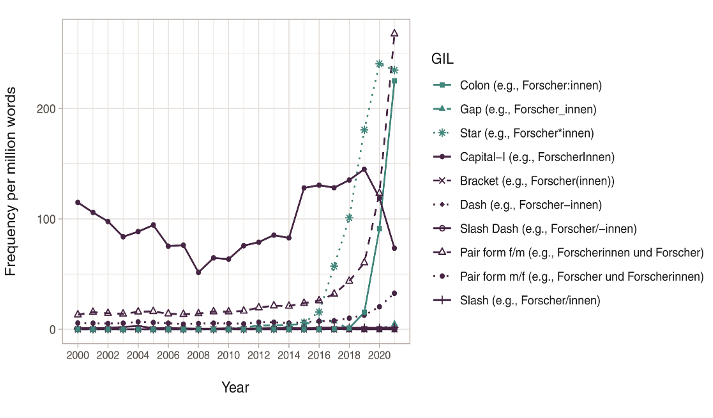
\includegraphics[width=1\textwidth]{gfl_types_frequency.png}
        \caption[Frequency of different types of gender-inclusive language]{Frequency of different types of gender-inclusive language. Source: \textcite{waldendorfWordsChangeIncrease2024} p. 367.}
        \label{fig:gfl_types_frequency}
    \end{figure}

    \subsubsection{Challenge of Integrating Gender-Fair Language into NLP}
    The use of GFL has increased in recent years \parencite{waldendorfWordsChangeIncrease2024}, but it remains generally low. This results in a scarcity of relevant linguistic data. Few datasets include GFL variants, and existing resources often rely on manual translations or post-editing to add gender-inclusive forms \parencite{lardelliBuildingBridgesDataset2024}. For this project, the limited availability of GFL data poses a significant challenge, especially when training the model to recognize gender-fair alternatives as neutral due to the lack of consistent examples.

    % --------------------------------------------------------------------------------

    \subsection{Research Gaps}
    A central gap in gender bias research is the absence of a shared definition of what constitutes "fair" language. This lack of conceptual clarity makes it difficult to design systematic evaluation approaches, define accountability standards, or detect all relevant forms of harm \parencite{barclayInvestigatingMarkersDrivers2024a,shresthaExploringGenderBiases2022,stanczakSurveyGenderBias2021}.

    A second major gap concerns the availability of high-quality EN-DE translation data that includes GFL. This limits the development and evaluation of models that aim to identify biased output in a structured and reproducible way. While a few datasets exist, they are not designed for bias detection tasks and often require manual post-editing to incorporate inclusive forms \parencite{lardelliBuildingBridgesDataset2024}.

    \textcite{stanczakSurveyGenderBias2021} show that findings on gender bias in English do not always apply to other languages like German. Linguistic differences make language-specific approaches necessary to address fairness in MT. Studies on EN-DE systems \parencite{ullmannGenderBiasMachine2022,kapplAreAllSpanish2025,lardelliBuildingBridgesDataset2024} confirm the presence of gender bias, suggest mitigation strategies, or introduce evaluation metrics. Yet, only a few focus on systematic methods to detect bias in translated text.

   This project addresses that gap by focusing on bias detection as a foundational step. Because reliable automatic debiasing is not yet available, manual correction will likely still be needed. The focus remains on identifying biased translations rather than fixing them.

% --------------------------------------------------------------------------------

\section{Approach and Justification of the Technical Setup}
    This section outlines the technical setup used in the project and explains the rationale behind design choices. It also provides background information on the underlying technologies to clarify how each component contributes to the overall goal of detecting gender bias in EN-DE translations.

\subsection{Binary Classification in NLP}
    Binary classification means sorting items into two clear groups. It is the most common task in ML and is frequently found in every day life, such as automatically flitering e-mails as "spam" or "not spam" \parencite{quemyBinaryClassificationUnstructured2019} or deciding whether a transaction is "fraudulent" or "legitimate". For instance, a spam filter uses previously labeled e-mails to learn relevant patterns, such as specific keywords or sender information, and builds a model that applies these patterns to classify new messages accurately. 
    
    This thesis tries to label a translation as either "biased" or "neutral". While it is possible to extend the classification beyond two categories, such as distinguishing types of bias or including labels like "gender-fair", this would require much more data and training. Given the practical aim of this work, which is to help users quickly identify whether their text might contain gender bias, the model focuses on a simple binary decision.

\subsection{Transformer Architecture} \label{subsection:transformer_arch}
  To provide some background on the BERT architecture, it is important to understand its foundation in the Transformer model. The Transformer is designed to process input sequences and \textit{transform} them into output sequences. To do this effectively, it uses a self-attention mechanism \parencite{phuongFormalAlgorithmsTransformers2022}.

    \subsubsection{Self-attention mechanism}
    The self-attention mechanism allows the model to weigh the significance of all input elements simultaneously \parencite{xiaoIntroductionTransformersNLP2023}, meaning it can look at all words in a sentence at once and decide which ones are most relevant to each word. Unlike traditional methods like Recurrent Neural Networks (RNNs), which process input step by step, self-attention captures global dependencies and contextual relationships more accurately, creating "context-aware" representations.

    \subsubsection{Encoder-Decoder Framework} \label{subsection:encoder-decoder}
    The transformer architecture consists of two main components: the encoder and the decoder. The encoder’s job is to read the input sentence and turn it into a series of vectors the model can understand. Each vector is a list of numbers representing the meaning and structure of each word \parencite{xiaoIntroductionTransformersNLP2023}. The encoder works as follows (see \autoref{fig:transformer_architecture}):

    \begin{enumerate}
        \item It receives input embeddings, which represent the words, and positional encodings, which tell the model the order of the words.
        
        \item The data then passes through several identical layers. Each layer has two main components. Each of these is followed by an \textbf{Add \& Layer Norm} step, which helps stabilize and preserve useful information:
        \begin{enumerate}[label=\alph*.]
            \item \textbf{Multi-head self-attention} runs several attention processes in parallel. Each attention head focuses on different details to help the model understand the sentence better.
            \item A \textbf{Feed-forward network} processes each word vector separately, refining the information like a small filter.
    \end{enumerate}
    
    \item Each layer builds on the output of the previous one, helping the model form more complex and abstract ideas about the input sentence.
    
    \item Finally, the encoder outputs a sequence of \textit{hidden states}. These are continuous vector representations for each input token. They encode contextual information from the entire sentence. For example, in the sentence "The cat sat on the mat," the vector for "cat" reflects its relationship to words like "sat" and "mat."
\end{enumerate}

\begin{figure}[ht]
    \centering
	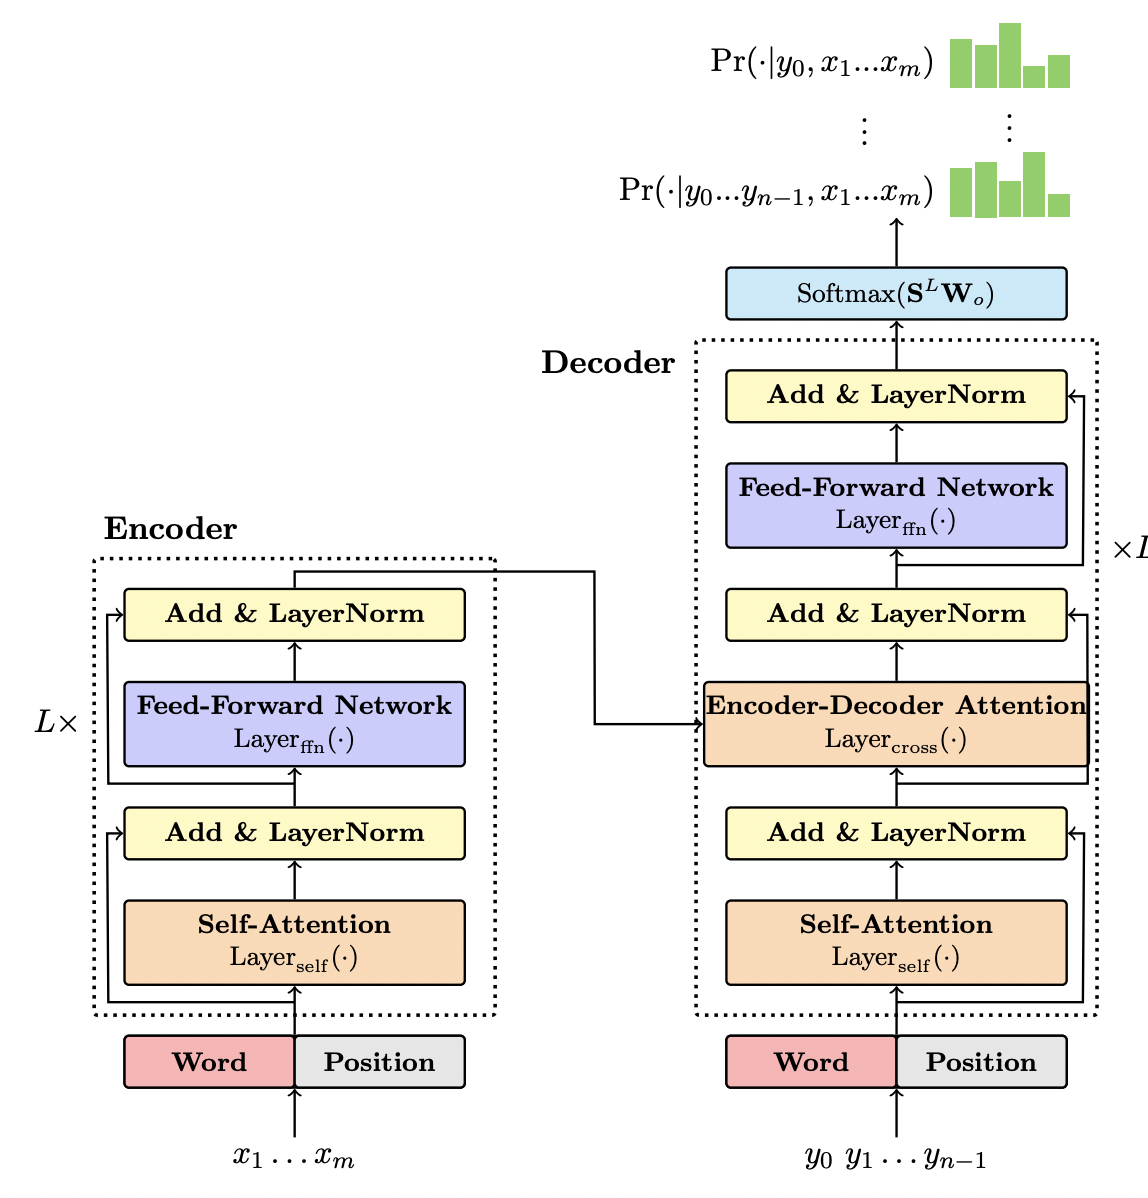
\includegraphics[width=\textwidth,height=0.45\textheight,keepaspectratio]{transformer_architecture.png}	
        \caption[Transformer encoder-decoder architecture overview]{Transformer encoder-decoder architecture. The encoder (left) processes input tokens \(x_1,\dots,x_m\) through: (1) a self-attention layer for contextual relationships, (2) a feed-forward network for feature transformation, and (3) residual connections with layer normalization. The decoder (right) generates outputs by attending to both the encoder's representations and its previous outputs ($y_0$ to $y_{n-1}$), producing the next-token probability distribution. Figure and description adapted from \textcite{xiaoIntroductionTransformersNLP2023}, p. 6.}
    \label{fig:transformer_architecture}
\end{figure}

The decoder generates the output sentence one word at a time by using the information from the encoder \parencite{xiaoIntroductionTransformersNLP2023}. However, since BERT uses only an encoder-only architecture (see \autoref{fig:bert_arch}), the decoder is not relevant for this work and is therefore excluded from the discussion.

\subsection{BERT}
    BERT is a language model that stands for "Bidirectional Encoder Representations from Transformers" and was introduced by Google in 2018 \parencite{devlinBERTPretrainingDeep2019}. After pre-training, BERT can be adapted to many NLP tasks by adding a simple output layer and fine-tuning, without needing major changes to its design. Since BERT uses only the encoder part of the Transformer architecture, it is designed to understand input rather than generate output. This makes it especially suitable for a binary classification task, where the goal is to analyze input texts and assign it to one of two categories.

    There are multiple variants of the original BERT model. It was originally released in two sizes: \texttt{BERT-Base} and \texttt{BERT-Large}, which differ in the number of layers, attention heads, and overall model capacity \parencite{devlinBERTPretrainingDeep2019}. Since then, many other versions have been developed. Most of them modify either BERT’s pre-training objectives or the underlying Transformer architecture \parencite{libovickyHowLanguageNeutralMultilingual2019}.

\subsection{Multilingual BERT (mBERT)}
    For this thesis, I use multilingual BERT \textbf{\href{https://huggingface.co/google-bert/bert-base-multilingual-cased}{(\texttt{mBERT})}} \parencite{devlinBERTPretrainingDeep2019}. \texttt{mBERT} uses the same configuration as \texttt{BERT-Base}, but it is pretrained on Wikipedia data from 104 languages, including both English and German. 
    
    The model does not receive any explicit signal about which language it is processing. It is also not trained to align translations across languages. Instead, its multilingual ability emerges from shared patterns it learns across the multilingual corpus \parencite{piresHowMultilingualMultilingual2019}. Despite the lack of cross-lingual supervision, the model develops internal representations that support tasks in multiple languages.

    Monolingual models like \href{https://huggingface.co/google-bert/bert-base-german-cased}{\texttt{German BERT}} do not support English input. Larger multilingual models, such as \href{https://huggingface.co/docs/transformers/en/model_doc/xlm-roberta}{\texttt{XLM-RoBERTa}}, require more computational resources and training time, which was not feasible here. \texttt{mBERT} offers a good balance between language coverage, model size, and training efficiency, making it a practical choice detecting gender bias in EN-DE translations.

\begin{figure}
    \centering
	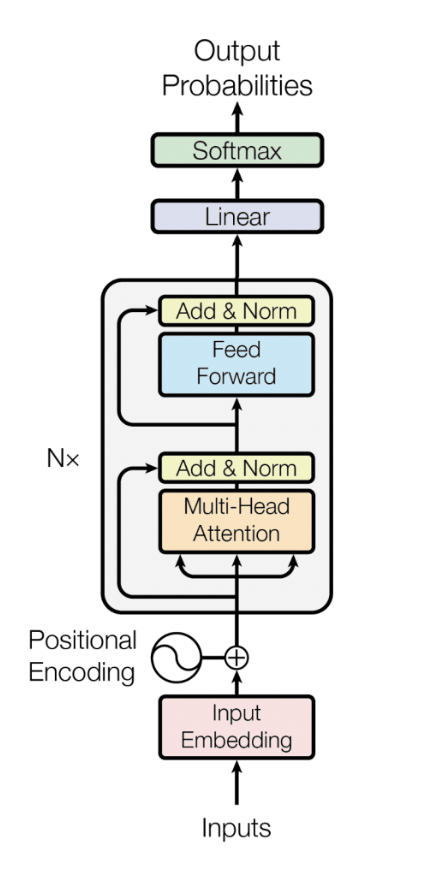
\includegraphics[width=\textwidth,height=0.45\textheight,keepaspectratio]{BERT_architecture.png}	
    \caption[BERT's encoder-only architecture].{BERT's encoder-only architecture Figure by \textcite{smithCompleteGuideBERT2024}.}
    \label{fig:bert_arch}
\end{figure}

\subsubsection{Tokenization}
\texttt{mBERT} processes input by splitting words or subword units into \textit{tokens} (tokenization)\footnote{This tokenization process applies to both BERT and mBERT.}. It uses the WordPiece algorithm with a shared vocabulary of 110,000 tokens, and all texts are lowercased before tokenization \parencite{devlinMultilingualBERTGitHub2018}. To balance the training data, languages with large Wikipedia corpora are downsampled, while those with fewer resources are oversampled.

Pre-processing is the same for all supported languages: (1) converting text to lowercase and removing accents, (2) splitting punctuation, and (3) tokenizing based on whitespace. Removing accents helps reduce the vocabulary size, even though it can introduce ambiguity in languages where accents carry meaning. This trade-off is accepted because \texttt{mBERT's} contextual embeddings usually resolve such ambiguities during training and inference.

Special tokens are reserved units added to the input text to mark structure. They are not real words but placeholders that tell the model how to interpret different parts of the input.

\begin{itemize}
	\item \texttt{[CLS]} (classification) marks the start of the sequence,
	\item \texttt{[SEP]} separates sentence pairs.
\end{itemize}

\noindent In this work, each input combines an English source sentence and its German translation as:

\begin{quote}
    \texttt{[CLS] english sentence [SEP] german translation [SEP]}
\end{quote}

\begin{quote}
\texttt{[CLS] the nurse is kind [SEP] die krankenschwester ist nett [SEP]}
\end{quote}

\subsubsection{Mechanics of Fine-Tuning mBERT}
    Fine-tuning adjusts the base model for a specific task, in this case, detecting gender bias in translations.\footnote{This fine-tuning process applies to both BERT and mBERT.} To do so, a new labeled dataset is used to continue training the model, allowing it to adapt its weights to task-specific patterns. 

    A classification head is an additional layer added to the top of the model to turn its general language understanding into task-specific predictions. It usually consists of a linear layer, which transforms the model’s output into a set of scores, followed by a softmax function, which converts these scores into probabilities for each class.

    In this case, the classification head uses the final hidden state of the \texttt{[CLS]} as the input. The linear layer maps this vector to two values (biased or not biased), and the softmax function outputs the probability for each class.

    \[
    z = Wx + b
    \]

    Here, \(x\) is the \texttt{[CLS]} embedding, \(W\) is the weight matrix, and \(b\) is the bias vector. Both \(W\) and \(b\) are parameters learned during training to help map \texttt{mBERT’s} output to the task labels. This changes the output into two numbers (logits), one for each class: biased or neutral. Then, the softmax function turns these numbers into probabilities \parencite{devlinBERTPretrainingDeep2019,xiaoIntroductionTransformersNLP2023}. Short for "soft maximum," it maps raw scores to a probability distribution, emphasizing the highest values while still giving smaller ones some weight.

    \[
    \text{softmax}(z_i) = \frac{e^{z_i}}{\sum_{j=1}^{K} e^{z_j}}
    \]

    Each logit \( z_i \) is exponentiated to ensure positivity. The result is then normalized by dividing by the sum of all exponentials, producing the probability distributions. \( K \) is the number of possible classes. The class with the highest probability is selected as the model’s prediction.
    
\subsubsection{Key Hyperparameters Explained} \label{subsection:hyperparameters_explained}
    Fine-tuning can be unstable, and changes such as different seeds can lead to large differences in task performance \parencite{mosbachStabilityFinetuningBERT2021}. Tuning a set of key hyperparameters is therefore necessary. These are not learned by the model but must be set manually or through experimentation. Their values affect how fast the model learns, how stable training is, and how well the model generalizes to new data.

    The \textit{learning rate} controls how much the model updates its weights during each step \parencite{mosbachStabilityFinetuningBERT2021}. If it is too high, the model may not converge and instead jump over good solutions. If it is too low, training can be very slow or get stuck in local minima.

    \textit{Warmup steps} are used at the beginning of training to gradually increase the learning rate from zero to its target value \parencite{mosbachStabilityFinetuningBERT2021}. This helps avoid instability in the early stages, where large updates can be harmful. After the warmup period, the learning rate is often decreased again using a scheduler, which controls how it changes over time.

    The \textit{number of epochs} defines how many times the model passes through the entire training dataset \parencite{mosbachStabilityFinetuningBERT2021}. More epochs mean more training iterations, which can help the model better fit the data. On small datasets, training for more epochs—sometimes up to 20 instead of the usual 3—helps reduce instability and improves generalization. This is because the model has more chances to learn meaningful patterns instead of stopping too early.

    The \textit{batch size} refers to how many training examples the model processes before updating its parameters \parencite{mosbachStabilityFinetuningBERT2021}. Commonly, a batch size of 16 is used during fine-tuning \texttt{mBERT}. Larger batches provide more stable gradient estimates but require more memory. Smaller batches can introduce noise in the updates but might help the model generalize better. While \textcite{mosbachStabilityFinetuningBERT2021} does not deeply analyze batch size effects on stability, it remains an important parameter to balance resource limits and training quality.

    Finally, the \textit{optimizer} controls how the model weights are adjusted to minimize prediction error \parencite{mosbachStabilityFinetuningBERT2021}. The AdamW optimizer is standard for \texttt{mBERT} fine-tuning because it adapts learning rates per parameter and includes weight decay regularization. A critical feature of Adam is \textit{bias correction}, which reduces the effective learning rate early in training. This acts like an implicit warmup, preventing large unstable updates and vanishing gradients in the lower layers. Combining explicit warmup with Adam’s bias correction allows training with higher learning rates more stably.

    \vspace{0.6em}
    \begin{table}[h]
        \centering
        \begin{tabularx}{\textwidth}{l X}
        \toprule
        \textbf{Hyperparameter} & \textbf{Role in Fine-Tuning} \\
        \midrule
        Learning Rate & Controls how much model weights are updated at each step; too high causes instability, too low slows training. \\
        Warmup Steps & Gradually increases the learning rate at the start to prevent unstable early updates. \\
        Number of Epochs & Defines how many times the model sees the full training data; more epochs help on small datasets. \\
        Batch Size & Number of samples processed before an update; affects stability, memory use, and generalization. \\
        Optimizer & Algorithm for updating weights; AdamW is standard, with adaptive rates and weight decay. \\
        \bottomrule
        \end{tabularx}
        \caption{Summary of key hyperparameters used during fine-tuning.}
    \end{table}


\subsubsection{Layer Freezing During Fine-Tuning} \label{subsection:layer_freezing}
    Layer freezing refers to the practice of keeping certain layers of a pretrained model fixed during fine-tuning, meaning their weights are not updated. This approach reduces the number of trainable parameters. This not only speeds up training \parencite{sorrentiSelectiveFreezingEfficient2023} but also helps prevent overfitting on small datasets and preserves the broad language knowledge from pre-training.

    In monolingual BERT, lower layers typically encode general syntactic and semantic patterns, while higher layers are more task-specific \parencite{nadipalliLayerWiseEvolutionRepresentations2025}. As a result, it is common to freeze the lower layers and only fine-tune the top layers and the classification head, especially in resource-constrained settings \parencite{nadipalliLayerWiseEvolutionRepresentations2025}.

    In \texttt{mBERT}, the distribution of cross-lingual and language-specific features across all layers makes layer freezing less straightforward. \textcite{wuBetoBentzBecas2019} highlight that no single layer consistently captures the most relevant cross-lingual information, and even individual layers can perform well on sentence-level tasks. They suggest that freezing the lower six layers may improve generalization, but emphasize that optimal strategies depend on the specific task and require empirical testing \parencite{wuBetoBentzBecas2019}.

\subsubsection{Limitations of mBERT}
    One major limitation of \texttt{mBERT} is the "curse of multilinguality" \parencite{gurgurovMultilingualLargeLanguage2024}. Because it must represent 104 languages within a fixed parameter budget, the capacity available per language is limited. This causes reduced performance across languages compared to monolingual models. Even high-resource languages like English perform worse in \texttt{mBERT} than in their dedicated BERT models. Additionally, the shared vocabulary of 110,000 tokens is diluted, meaning it is less tailored to any single language. Languages with more data tend to get better performance, while others suffer.

    Since \texttt{mBERT} is pretrained on Wikipedia, it reflects biases inherent to that corpus. German Wikipedia articles predominantly use the generic masculine \parencite{sichlerGenderDifferencesGermanlanguage2014}, while gender-fair alternatives appear only sporadically, mostly in discussions or articles about female-dominated professions. These biases can influence the model’s outputs and are especially important to consider in a gender bias detection context.

    Despite these limitations, \texttt{mBERT} remains the most fitting choice for this thesis. Since I work with English and German, which are both high-resource and related languages, \texttt{mBERT} generally performs better than it would with low-resource languages or languages from distant language families with fewer similarities \parencite{lauscherZeroHeroLimitations2020}.

\subsection{Chosen Evaluation Metrics}
    Evaluation metrics quantify how effectively the model identifies gender bias. They provide objective measures to assess and compare performance.

    In this task, it is particularly important to minimize two types of errors: false positives, where unbiased translations are mistakenly identified as biased, and false negatives, where genuine instances of bias are overlooked. A model that resorts to random guessing or consistently avoids flagging bias lacks practical value.

    The metrics that capture these errors are precision and recall \parencite{rainioEvaluationMetricsStatistical2024}:

\begin{itemize}
    \item \textbf{Precision:} Of all translations flagged as biased, how many truly are biased? High precision means fewer false alarms.
    \item \textbf{Recall:} Of all biased translations, how many did the model correctly detect? High recall means fewer missed biases.
\end{itemize}

There is often a trade-off between precision and recall. A model with high precision but low recall misses many real biases, while one with high recall but low precision raises too many false warnings. To balance this trade-off, the F1 score is used. It combines precision and recall into a single number by calculating their harmonic mean:

\[
F1 = 2 \cdot \frac{\text{Precision} \cdot \text{Recall}}{\text{Precision} + \text{Recall}}
\]
\vspace{0.5em}

\subsection{Interactive Demo}
    The fine-tuned model is intended to be presented through an interactive demonstration. Since the focus lies on showcasing the model’s functionality rather than creating a fully developed application, \href{https://streamlit.io/}{Streamlit} was chosen. Streamlit allows for quick and easy development of lightweight user interfaces in Python, providing a simple setup and effective performance. For live translation, an open-source tool supporting EN-DE pairs was required. \href{https://github.com/Helsinki-NLP/Opus-MT}{Opus-MT} \parencite{tiedemannOPUSMTBuildingOpen2020} meets these criteria and integrates smoothly into the demonstration. While state-of-the-art translators like Google Translate or DeepL would have been preferred for their quality, they do not meet the requirements for this setup. Therefore, a separate tab for manual translation input was added, allowing users to paste translations directly and bypass this limitation.

\subsubsection{Chapter Summary}
    This chapter reviewed related work to map the current research landscape and identify key gaps. A major gap is the absence of robust detection systems for gender bias in EN-DE MT. While prior studies confirm the presence of bias and suggest mitigation strategies, few offer systematic methods or tools to reliably identify biased translations. Another key issue is the lack of a shared definition of “fair” language or gender bias, which complicates evaluation, accountability, and the design of detection models.

    I address this by focusing on detection as a first step and building a task-specific dataset from existing resources. Since there is no shared definition of gender bias, I define two common patterns that the system targets. The chapter also introduced key technical concepts needed understand the following methodology chapter.